% gc-15-IntLab.tex

\documentclass[xcolor=dvipsnames]{beamer}

\usepackage{cancel}
\renewcommand{\CancelColor}{\color{red}}
\usepackage{graphicx}
\usepackage{wrapfig}
\usepackage{colortbl}
\usepackage{color}
\usepackage{alltt}
\definecolor{myblue}{rgb}{0.8,0.85,1}

\mode<presentation>
{
  \usetheme{Warsaw}
  \setbeamercovered{transparent}
}
% \usecolortheme[named=OliveGreen]{structure}
\setbeamertemplate{navigation symbols}{} 
\setbeamertemplate{blocks}[rounded][shadow=true] 

\newcounter{expls}
\setcounter{expls}{0}
\newcommand{\beispiel}[1]{\refstepcounter{expls}\textbf{Example \arabic{expls}: #1.}}

\newcounter{exercise}
\setcounter{exercise}{0}
\newcommand{\ubung}[0]{\refstepcounter{exercise}\textbf{Exercise \arabic{exercise}: }}

\newcommand{\eibe}{1}
\newcommand{\reeq}{2.5}
\newcommand{\aeza}{8.3}
\newcommand{\emah}{2.1}
\newcommand{\biet}{4.9}
\newcommand{\hohq}{Jane}
\newcommand{\wili}{She}
\newcommand{\ahhi}{she}
% \newcommand{\usax}{13}
\newcommand{\bohh}{her}
% \newcommand{\eiri}{\lim_{x\rightarrow\frac{\pi}{4}}\frac{\sin{}x-\cos{}x}{x-\frac{\pi}{4}}}
\newcommand{\kahr}{\lim_{x\rightarrow\frac{\pi}{2}}\frac{2x-\pi}{\cos{}x}}
% \newcommand{\ohdo}{0.4}
% \newcommand{\eigh}{1.4}
% \newcommand{\hahs}{\int\left(\frac{\sqrt{x}}{2}+\frac{2}{\sqrt{x}}\right)\,dx}
\newcommand{\ooce}{\int_{0}^{\pi}7.5\sin{}x\,dx}
% \newcommand{\sheq}{2}

% \newcommand{\eibe}{2}
% \newcommand{\reeq}{2.2}
% \newcommand{\aeza}{7.5}
% \newcommand{\emah}{1.9}
% \newcommand{\biet}{5.1}
% \newcommand{\hohq}{Shane}
% \newcommand{\wili}{He}
% \newcommand{\ahhi}{he}
\newcommand{\usax}{11}
% \newcommand{\bohh}{his}
\newcommand{\eiri}{\lim_{x\rightarrow\frac{\pi}{3}}\frac{\cos{}x-0.5}{x-\frac{\pi}{3}}}
% \newcommand{\kahr}{\lim_{t\rightarrow0}\frac{\sin{}t^{2}}{t}}
\newcommand{\ohdo}{0.7}
\newcommand{\eigh}{1.7}
\newcommand{\hahs}{\int\left(\sqrt{x}+\sqrt[3]{x}\right)\,dx}
% \newcommand{\ooce}{\int_{0}^{\pi}8.5\sin{}x\,dx}
\newcommand{\sheq}{3}

\newif\ifBCITCourse
\BCITCoursetrue
% \BCITCoursefalse
\newif\ifWhichCourse
\WhichCoursetrue
\WhichCoursefalse
\ifBCITCourse
\ifWhichCourse
\newcommand{\CourseName}{Statistics for Food Technology}
\newcommand{\CourseNumber}{MATH 2441}
\newcommand{\CourseInst}{BCIT}
\else
\newcommand{\CourseName}{Calculus for Geomatics}
\newcommand{\CourseNumber}{MATH 2511}
\newcommand{\CourseInst}{BCIT}
\fi
\else
\newcommand{\CourseName}{Philosophy and Literature}
\newcommand{\CourseNumber}{PHIL 375}
\newcommand{\CourseInst}{UBC}
\fi

\title{Lab for Integrals}
\subtitle{{\CourseNumber}, BCIT}

\author{\CourseName}

\date{March 31, 2017}

\begin{document}

\begin{frame}
  \titlepage
\end{frame}

\begin{frame}
  \frametitle{Integration Exercises I}
Find the following indefinite integrals.
\begin{equation}
  \label{eq:eevoomoh}
  \int{}6\,dx
\end{equation}
\begin{equation}
  \label{eq:eohauthu}
  \int{}-2\,dx
\end{equation}
\begin{equation}
  \label{eq:heizieta}
  \int{}8x^{4}\,dx
\end{equation}
\begin{equation}
  \label{eq:zohjieph}
  \int{}\pi{}x^{3}\,dx
\end{equation}
\begin{equation}
  \label{eq:oodaelad}
  \int{}\left(x^{3}+7-2x^{2}\right)\,dx
\end{equation}
\begin{equation}
  \label{eq:eeshooyo}
  \int{}\sqrt{x}\,dx
\end{equation}
\begin{equation}
  \label{eq:uafievai}
  \int{}\frac{7}{2}x^{\frac{5}{2}}\,dx
\end{equation}
\end{frame}

\begin{frame}
  \frametitle{Integration Exercises II}
Find the following indefinite integrals.
\begin{equation}
  \label{eq:igheivei}
  \int{}9\sqrt[5]{2x}\,dx
\end{equation}
\begin{equation}
  \label{eq:akahheju}
  \int{}\frac{3}{x^{3}}\,dx
\end{equation}
\begin{equation}
  \label{eq:zeifahce}
  \int{}\frac{7}{\sqrt[3]{x}}\,dx
\end{equation}
\begin{equation}
  \label{eq:afahthud}
  \int{}\sqrt{x}\left(3x-2\right)\,dx
\end{equation}
\begin{equation}
  \label{eq:desheiga}
  \int{}\left(x+1\right)^{2}\,dx
\end{equation}
\begin{equation}
  \label{eq:oongaiqu}
  \int{}\frac{4x^{2}-2\sqrt{x}}{x}\,dx
\end{equation}
\begin{equation}
  \label{eq:ahxiequo}
  \int{}\frac{x^{3}+2x^{2}-3x-6}{x+2}\,dx
\end{equation}
\end{frame}

\begin{frame}
  \frametitle{Definite Integrals Exercises}
Evaluate each definite integral.
\begin{equation}
  \label{eq:ufaetohm}
  \int_{1}^{2}x\,dx\hspace{1in}  \int_{-2}^{2}x^{2}\,dx
\end{equation}
\begin{equation}
  \label{eq:vahyooyi}
  \int_{1}^{3}7x^{2}\,dx\hspace{1in}  \int_{-2}^{2}3s^{4}\,ds
\end{equation}
\begin{equation}
  \label{eq:wohbuxoo}
  \int_{0}^{4}(x^{2}+2x)\,dx\hspace{1in}  \int_{1}^{e}\frac{1}{x}\,dx
\end{equation}
\begin{equation}
  \label{eq:ohgooquu}
  \int_{5}^{10}\sqrt{x}\,dx\hspace{1in}\int_{1}^{4}\frac{2+x^{2}}{\sqrt{x}}\,dx
\end{equation}
\begin{equation}
  \label{eq:yoocaitu}
  \int_{-1}^{2}(3u-2)(u+1)\,du\hspace{1in}\int_{\frac{\pi}{6}}^{\pi}\sin\vartheta{}\,d\vartheta
\end{equation}
\end{frame}

\begin{frame}
  \frametitle{Washer Method Exercise}
{\ubung} The region bounded by the curve $y=x^{2}+1$ and the line
$y=-x+3$ is revolved around the $x$-axis to generate a solid. Find the
volume of the solid.
\begin{figure}[h]
  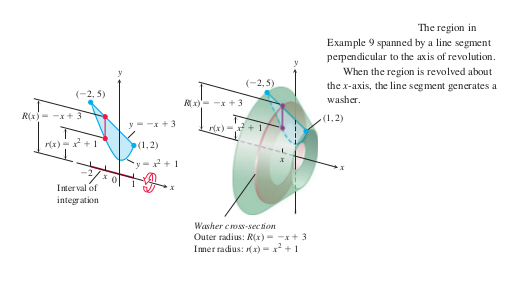
\includegraphics[scale=0.65]{./diagrams/washer.png}
\end{figure}
\end{frame}

\begin{frame}
  \frametitle{Washer Method Exercise}
{\ubung} The region bounded by the parabola $y=x^{2}$ and the line
$y=2x$ in the first quadrant is revolved about the $y$-axis to
generate a solid. Find the volume of the solid.
\begin{figure}[h]
  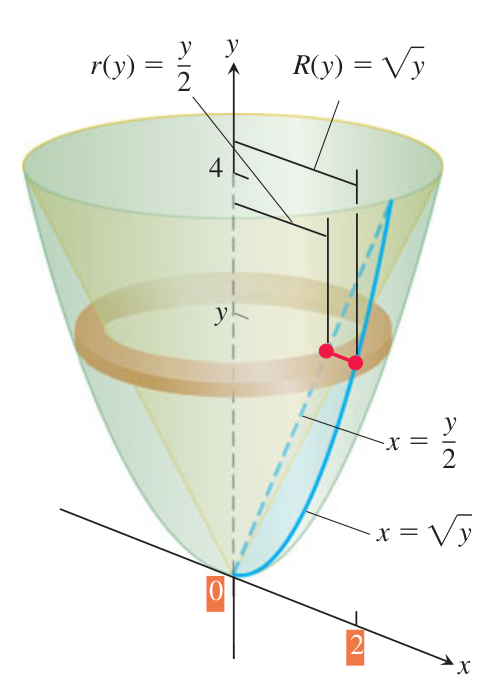
\includegraphics[scale=0.25]{./diagrams/radii.png}
\end{figure}
\end{frame}

\begin{frame}
  \frametitle{Exercises I}
% These exercises and the previous material are from S.T. Tan, Calculus
% for the Managerial, Life, and Social Sciences, p447.
Evaluate the following definite integrals.
\begin{equation}
  \label{eq:mauphouw}
  \int_{0}^{2}x(x^{2}-1)^{3}\,dx\hspace{1in}\int_{0}^{1}x^{2}(2x^{3}-1)^{4}\,dx
\end{equation}
\begin{equation}
  \label{eq:pahteeth}
  \int_{0}^{1}x\sqrt{5x^{2}+4}\,dx\hspace{1in}\int_{1}^{3}x\sqrt{3x^{2}-2}\,dx
\end{equation}
\begin{equation}
  \label{eq:ceiquoor}
  \int_{0}^{2}x^{2}(x^{3}+1)^{\frac{3}{2}}\,dx\hspace{1in}\int_{1}^{5}(2x-1)^{\frac{5}{2}}\,dx
\end{equation}
\begin{equation}
  \label{eq:riweevie}
  \int_{0}^{1}\frac{1}{\sqrt{2x+1}}\,dx\hspace{1in}\int_{0}^{2}\frac{x}{\sqrt{x^{2}+5}}\,dx
\end{equation}
\end{frame}

\begin{frame}
  \frametitle{Exercises II}
Evaluate the following definite integrals.
\begin{equation}
  \label{eq:aigighau}
  \int_{1}^{2}(2x+4)(x^{2}+4x-8)^{3}\,dx\hspace{1in}\int_{-1}^{1}x^{2}(x^{3}+1)^{4}\,dx
\end{equation}
\begin{equation}
  \label{eq:omixughu}
  \int_{0}^{2}xe^{x^{2}}\,dx\hspace{1in}\int_{0}^{1}e^{-1}\,dx
\end{equation}
\begin{equation}
  \label{eq:baemixeg}
  \int_{3}^{6}\frac{2}{x-2}\,dx\hspace{1in}\int_{0}^{1}\frac{e^{x}}{1+e^{x}}\,dx
\end{equation}
\begin{equation}
  \label{eq:aeteepah}
  \int_{0}^{1}\frac{x}{1+2x^{2}}\,dx\hspace{1in}\int_{1}^{2}\frac{\ln{}x}{x}\,dx
\end{equation}
\end{frame}

\begin{frame}
  \frametitle{Term Test B Problem 1} 
  {\hohq} is {\reeq} miles offshore in a boat and wishes to reach a
  coastal village {\aeza} miles down a straight shoreline from the
  point nearest the boat. {\wili} can row {\emah} miles per hour and
  can walk {\biet} miles per hour. Where should {\ahhi} land {\bohh}
  boat to reach the village in the least amount of time?
\end{frame}

\begin{frame}
  \frametitle{Term Test B Problem 2}
  An open-top box is to be made by cutting small congruent squares
  from the corners of a {\usax} inch by {\usax} inch sheet of tin and
  bending up the sides. How large should the squares cut from the
  corners be to make the box hold as much as possible?
\begin{figure}[h]
  \includegraphics[scale=0.5]{./diagrams/gc-termtestB-v\eibe-01.png}
\end{figure}
\end{frame}

\begin{frame}
  \frametitle{Term Test B Problem 3}
Evaluate the following limit.
\begin{equation}
  \label{eq:ahkisoav} \eiri\notag
\end{equation}

Evaluate the following limit.
\begin{equation}
  \label{eq:voolohqu} \kahr\notag
\end{equation}
\end{frame}

\begin{frame}
  \frametitle{Term Test B Problem 4}
To calculate a planet's space
coordinates, we have to solve equations like 
\begin{equation}
  \label{eq:aathieyi}
  x=1+{\ohdo}\sin{}x\notag
\end{equation}
Graphing the function $f(x)=x-1-{\ohdo}\sin{}x$
suggests that the function has a root near
$x={\eigh}$. Use one application of Newton's
method to improve this estimate. That is,
start with $x_{1}={\eigh}$ and find $x_{2}$.
\end{frame}

\begin{frame}
  \frametitle{Term Test B Problem 5}
Find the following indefinite
integral. 
\begin{equation}
  \label{eq:xieveimo}
  \hahs\notag
\end{equation}

Evaluate the following definite
integral.
\begin{equation}
  \label{eq:moubeing}
  \ooce\notag
\end{equation}
\end{frame}

\begin{frame}
  \frametitle{Term Test B Problem 6}
  Evaluate the following definite integral.
\begin{equation}
  \label{eq:gairooth}
  \int_{0}^{\sqrt{\sheq}}\left(t-\sqrt{\sheq}\right)\,dt\notag
\end{equation}
\end{frame}

\begin{frame}
  \frametitle{Additional Exercises}
  \begin{equation}
    \label{eq:esahtoip}
    \int\left(e^{3x}+5e^{-x}\right)\,dx
  \end{equation}
  \begin{equation}
    \label{eq:joopiemo}
    \int_{\ln{}2}^{\ln{}3}e^{x}\,dx
  \end{equation}
  \begin{equation}
    \label{eq:jelaenah}
    \int_{0}^{\frac{\pi}{4}}\left(1+e^{\tan{}\vartheta}\right)\sec^{2}\vartheta\,d\vartheta
  \end{equation}
  \begin{equation}
    \label{eq:pohchugh}
    \int\frac{e^{-\frac{1}{x^{2}}}}{x^{3}}\,dx
  \end{equation}
\end{frame}

\end{document}

